

\begin{figure}[htbp] \centering
  \caption{Aulas 1 e 2 Grupo 4 com 100\% de acerto}
  \label{fig: Aulas 1 e 2 - 100}
  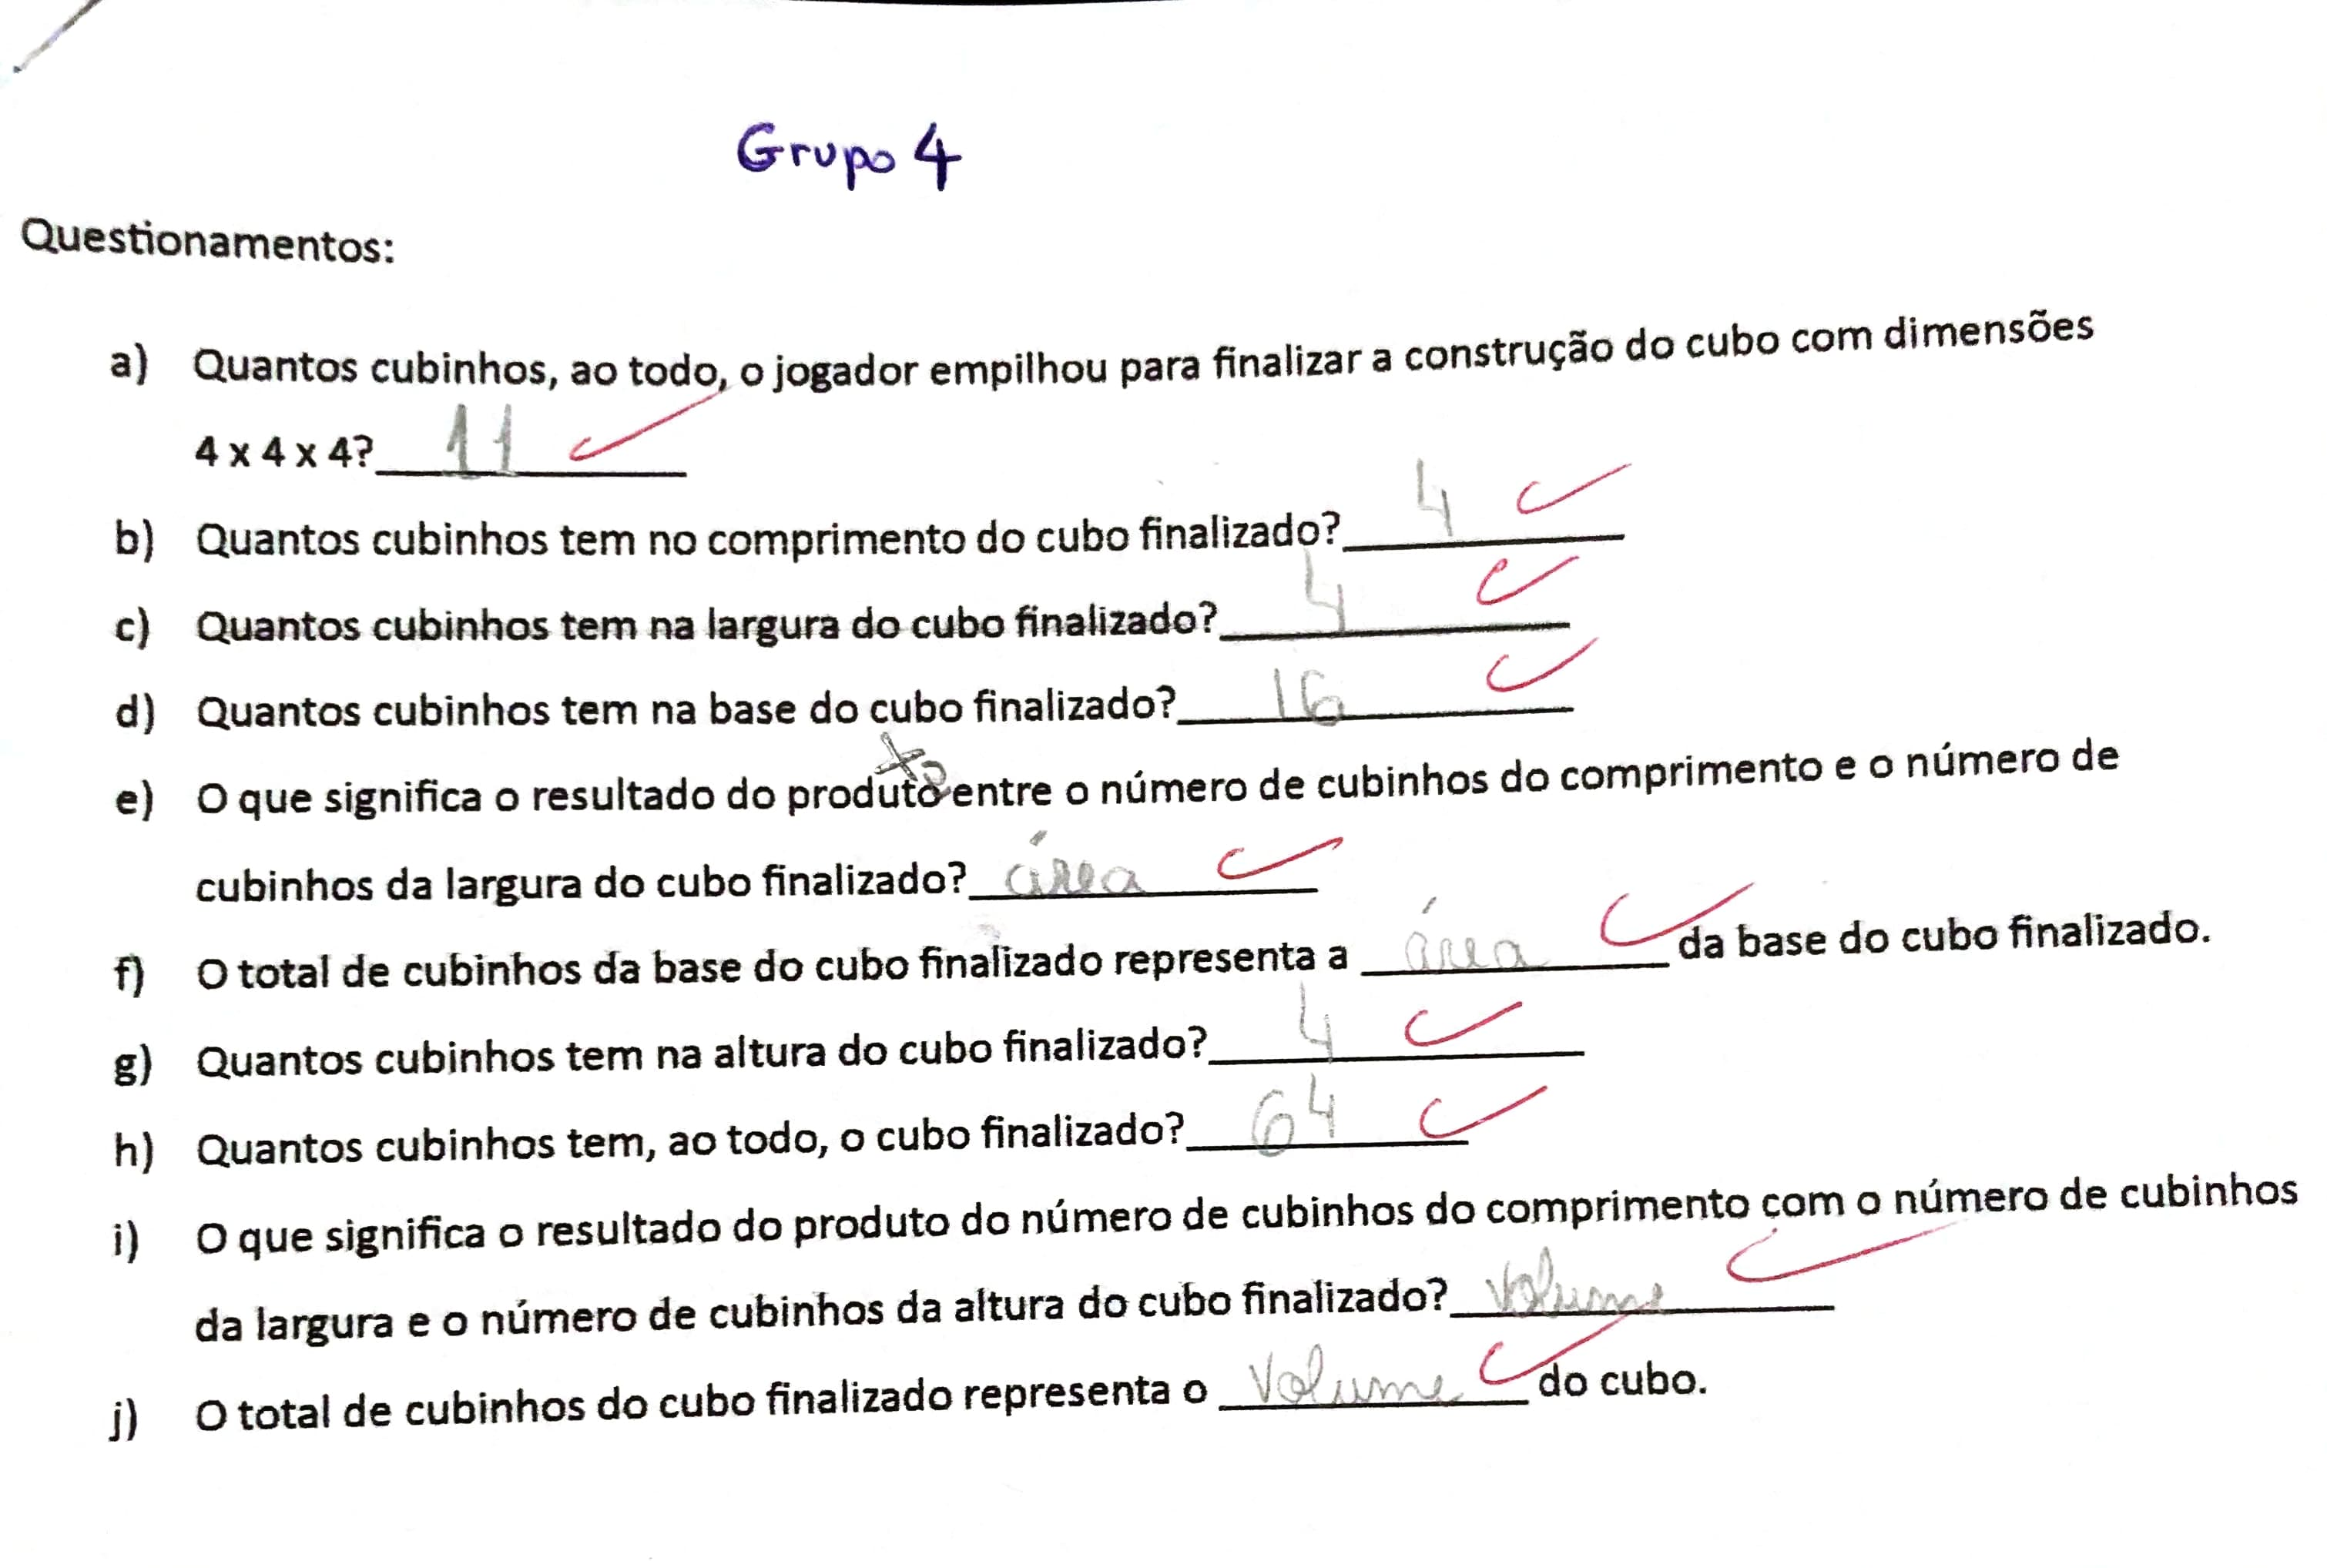
\includegraphics[width=0.5\linewidth]{Novas imagens/Grupo 4}
  \legend{\autoria}
\end{figure}

\begin{figure}[htbp] \centering
  \caption{Aulas 1 e 2 Grupo 1 com 40\% de acerto}
  \label{fig: Aulas 1 e 2 - 40}
  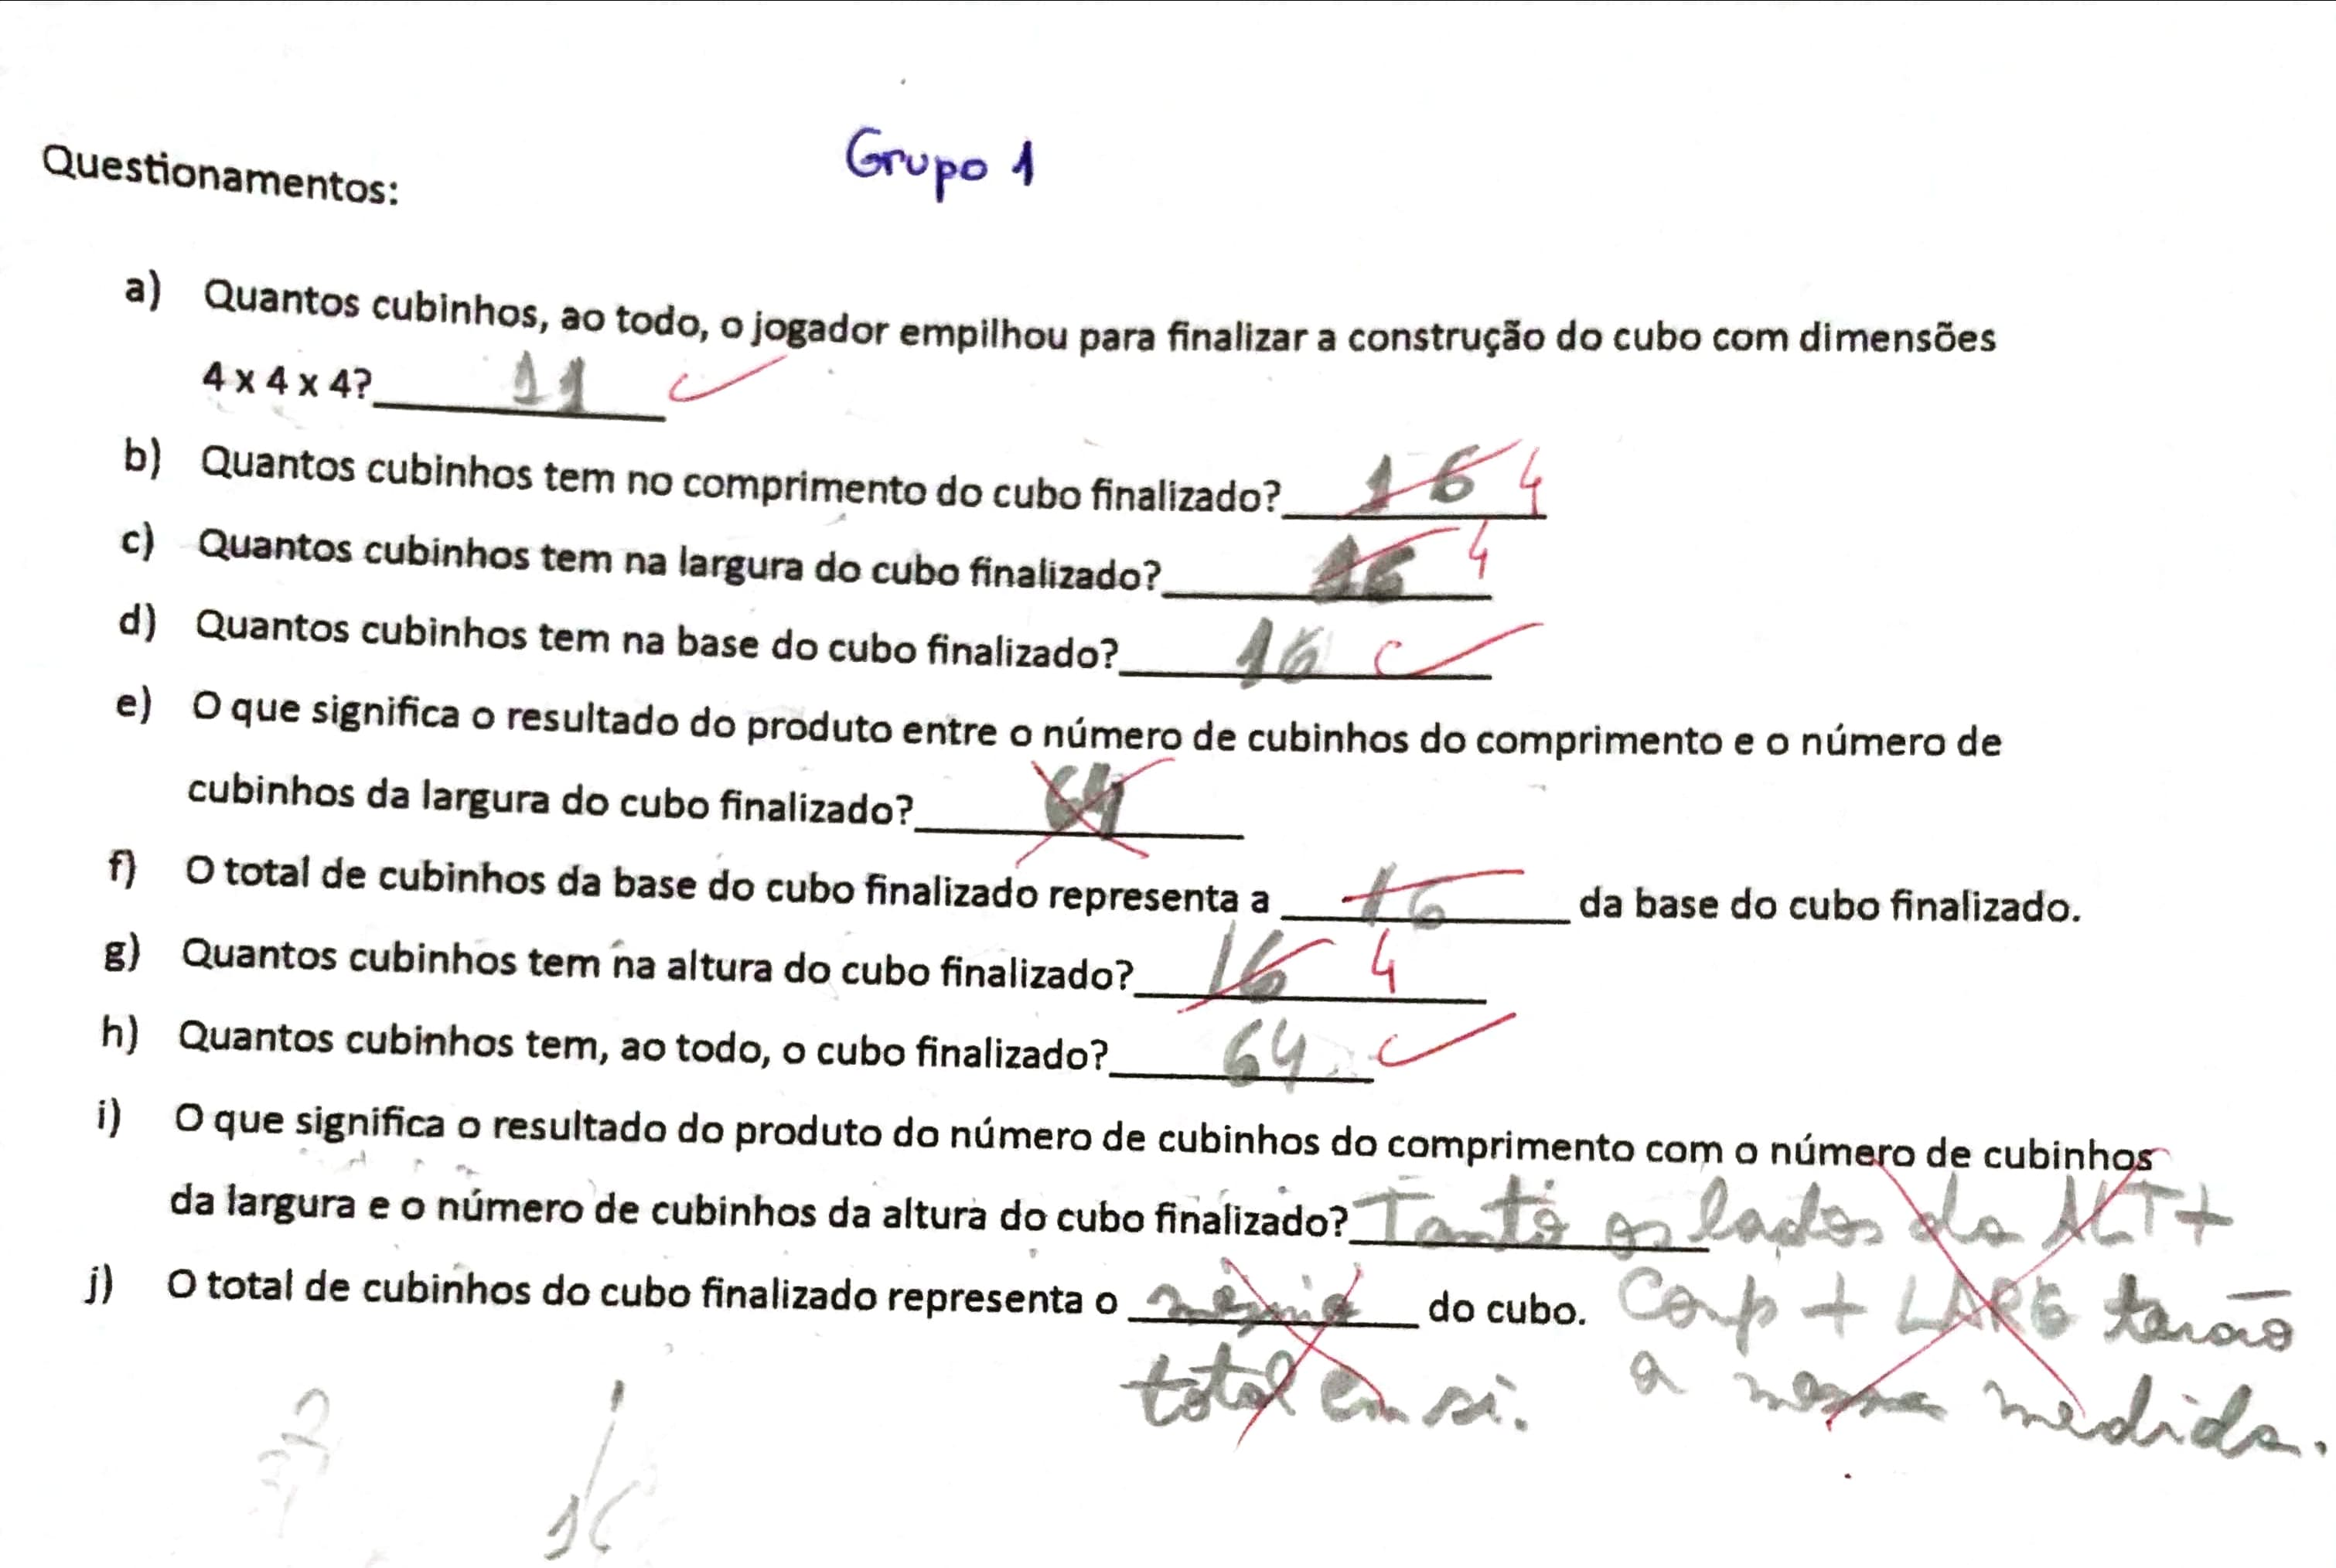
\includegraphics[width=0.5\linewidth]{Novas imagens/Grupo 1}
  \legend{\autoria}
\end{figure}

\begin{figure}[htbp] \centering
  \caption{Aulas 5 e 6 - Exercício 8}
  \label{fig:Aulas 5 e 6 - Exercício 8}
  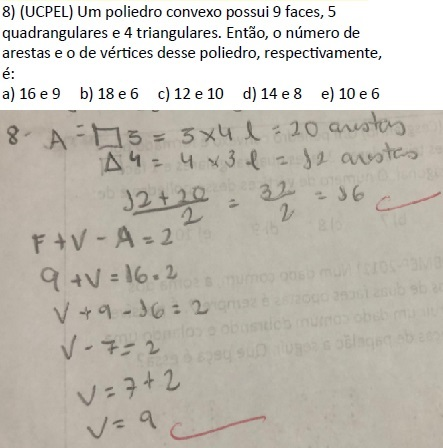
\includegraphics[width=0.5\linewidth]{Novas imagens/Exercício 8 Aulas 5 e 6}
  \legend{\autoria}
\end{figure}

\begin{figure}[htbp] \centering
  \caption{Sólidos Platônicos compilado}
  \label{fig: Sólidos Platônicos compilado}
  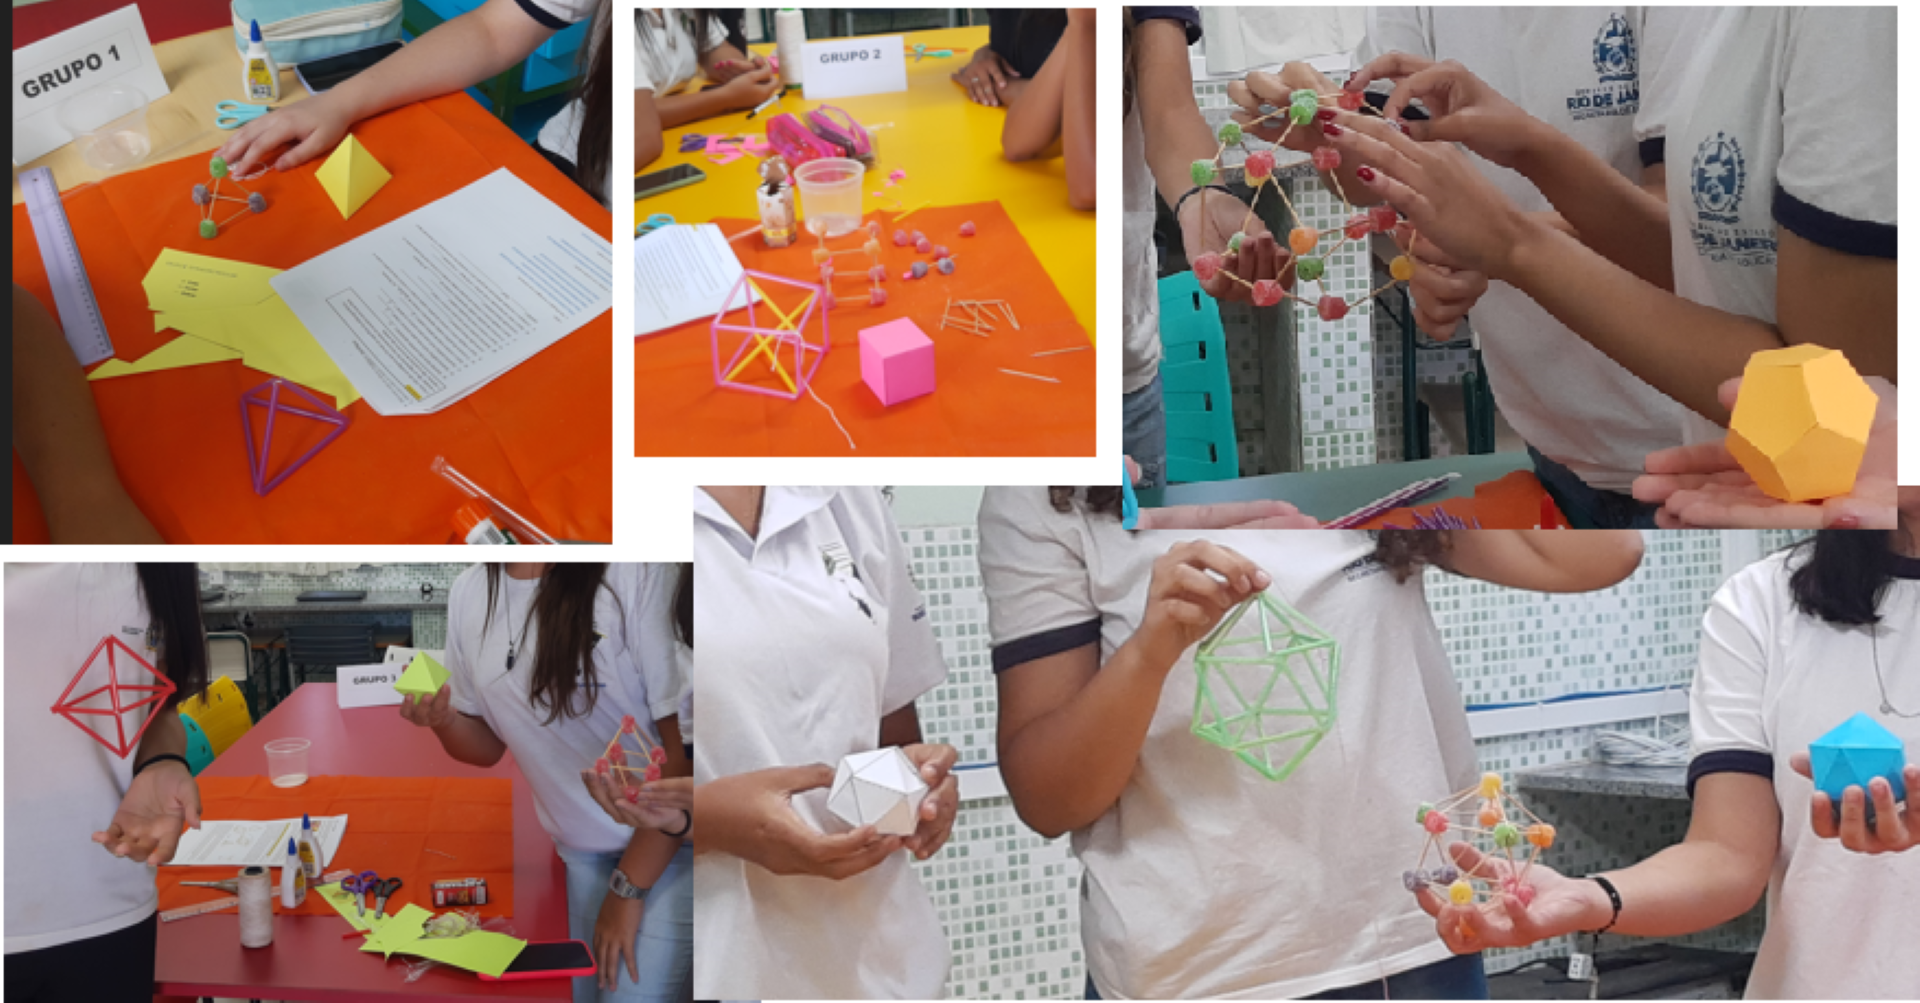
\includegraphics[width=0.5\linewidth]{Novas imagens/Sólidos Platônicos compilado}
  \legend{\autoria}
\end{figure}
